\documentclass[]{beamer}
\mode<presentation>{
  %% \usetheme[compress]{Berlin}
}
%% packages
\usepackage{zhspacing}
\zhspacing
\usepackage{graphics}
\usepackage{listings}
\lstset{
  basicstyle=\ttfamily\small,
  numbers=left
}
\usepackage{tabularx}
\usepackage{booktabs}
%% meta info
\title{Dataflow Analysis}
\subtitle{An Introduction}
\author[SuXing~pysuxing@gmail.com]{SuXing}
\institute{TOW}
\date{\today}

%% slides
\begin{document}
\setlength{\parindent}{0pt}

\frame{\titlepage}
\frame{\tableofcontents}

\section{Elements of Analysis}
\frame{\tableofcontents[currentsection]}

\begin{frame}
  \frametitle{Basic Conceptions}
  \begin{itemize}
    \item Concrete \& Abstract Values
    \item Lattice
    \item Abstraction Function
    \item Dataflow Infomation
    \item Flow Function
  \end{itemize}
\end{frame}

\begin{frame}
  \frametitle{Concrete Values}
  \alert{Concrete Vaules(CV)} are the values of variables in program execution,
  i.e. 0(Constant), \&a(memory address)

  \vspace{.5em}\pause
  \begin{columns}
    \begin{column}{.65\textwidth}
      \begin{tabular}{c|l}
        stmt & pointers\\
        \hline
        0 &  \\
        1 &  \\
        2 & p=\&i \\
        3 & p=\&i, q=NULL \\
        4 & p=\&i, q=NULL, s=uninitialized \\
        5 & p=\&i, q=NULL, s=uninitialized \\
        6 & p=\&i, q=NULL, s=\&i \\
        7 & p=\&i, q=NULL, s=uninitialized \\
        8 & p=\&i, q=NULL, s=NULL \\
        9 & p=\&i, q=NULL, s=?
      \end{tabular}
    \end{column}
    \begin{column}{.35\textwidth}
      \lstinputlisting[language=C]{listings/example.c}
    \end{column}
  \end{columns}
\end{frame}

\begin{frame}[t]
  \frametitle{Abstract Values}
  \alert{Abstract Values(AV)} are Concrete Values categorilized by characters to be tracked in
  dataflow analysis

  \only<2>{
    \begin{block}{Example}
      In null-dereference check, we find set of invalid ones in all defined pointers
      \centerline{int *p=\&a,*q=NULL,*s $\rightarrow$ \{q,s\}}
    \end{block}
  }

  \only<3->{
    \vspace{.5em}
    \begin{columns}
      \begin{column}{.65\textwidth}
        \begin{tabular}{c|cl}
          stmt & invalid pointers\\
          \hline
          0 & \{\} \\
          1 & \{\} \\
          2 & \{\} \\
          3 & \{q\} \\
          4 & \{q, s\} \\
          5 & \{q, s\} \\
          6 & \{q\} \\
          7 & \{q, s\} \\
          8 & \{q, s\} \\
          9 & \{q, s\}
        \end{tabular}
      \end{column}
      \begin{column}{.35\textwidth}
        \lstinputlisting[language=C]{listings/example.c}
      \end{column}
    \end{columns}
  }
  \only<4>{
    \vspace{.5em}
    \alert{Note} we analysis conservatively at statement 9!
  }
\end{frame}

\begin{frame}
  \frametitle{Lattice}
  To be correct, we make the analysis more appoximate, which means we are losing precision.

  \vspace{1em}\pause
  A \alert{Lattice} $L=(V, \sqsubseteq, \sqcup)$ is an algebra structure defined on domain $V$ with a
  \alert{partial order} $\sqsubseteq$ and a \alert{join operator} $\sqcup$.

  \vspace{1em}\pause
  There exists a \alert{top} element $\top$ and a \alert{bottom} element $\perp$ in $V$ that satisfies
  $$\forall \mu \in V, \mu \sqsubseteq T and \perp \sqsubseteq \mu$$

  \vspace{1em}\pause
  The join operator $\tau = \mu \sqcup \nu$ is defined as the minimal element in set
  $$\{\tau | \mu \sqsubseteq \tau, \nu \sqsubseteq \tau\}$$
\end{frame}

\begin{frame}
  \frametitle{Abstration Function}
  \alert{Abstration Function} is a map from Concrete Values to abstract values
  $$\alpha : CV \rightarrow AV$$

  \vspace{1em}\pause
  Often, we extend AV to a Lattice, so Abstract Function becomes
  $$\alpha : CV \rightarrow L$$
\end{frame}

\begin{frame}
  \frametitle{Dataflow Infomation}
  \alert{Dataflow Infomation} $\sigma$ is a map from program varialbles(Var) to abstract values.
  It's cosumed and generated by the analysis procedure
  $$\sigma : Var \rightarrow L$$

  \vspace{1em}\pause
  We annotate $\sigma$ with an integer representing the statment at which the analysis is done
  $$\sigma_i : Var \rightarrow L$$
\end{frame}

\begin{frame}
  \frametitle{Flow Function}
  A \alert{Flow Function} $f$ is the actual procedure doing analysis, it takes a statment(implicitly)
  and an input dataflow infomation and generate an output dataflow infomation
  $$f(\sigma_i) \rightarrow \sigma_{i+1}$$
\end{frame}

\section{Applications}
\frame{\tableofcontents[currentsection]}

\begin{frame}
  \frametitle{Null-Dereference Analysis}
  In Null-Dereference Analysis, we have
  \begin{itemize}
    \item $L=(V, \sqsubseteq, \sqcup)$ where
      \begin{itemize}
      \item $V=\{p | p is a pointer already declared\}$
      \item $\top = V$
      \item $\perp = \emptyset$
      \item $\sqsubseteq = \subseteq$
      \item $\sqcup = \cup$
      \end{itemize}
    \item $\sigma_0 = \emptyset$
    \item flow function $f_{ND}$ is trivial
  \end{itemize}
\end{frame}

\begin{frame}
  \frametitle{Zero Analysis}
  In Zero Analysis, we have
  \begin{itemize}
    \item $L=(V, \sqsubseteq, \sqcup)$ where
      \begin{itemize}
      \item $V=\{Z, N, anyvalue, unknown\}$
      \item $\top = anyvalue$
      \item $\perp = unknown$
      \item $unknown \sqsubseteq Z \sqsubseteq any-value, unknown \sqsubseteq N \sqsubseteq anyvalue$
      \item $unknown \sqcup Z = Z, unknown \sqcup N = N, Z \sqcup N = anyvalue$
      \end{itemize}
    \item $\sigma_0(\mu) = unknown$
    \item flow function $f_{ND}$ is trivial
  \end{itemize}
\end{frame}

\section{Implementation}
\frame{\tableofcontents[currentsection]}

\begin{frame}
  \frametitle{Iterative Approach}
  Intuitively, we start analysing from the first statment and go along with CFG path until
  a \alert{fixed point} is reached (the analysis
  information $\sigma_i$ we get at each statement does not change any more)

  \vspace{1em}\pause
  The analysis is guaranteed to terminate if the lattice $L$ and flow function $f$ fulfills
  some requirements, in whatever order the statements are analysised.
\end{frame}

\begin{frame}
  \frametitle{The Worklist Algorithm}
  The Worklist Algorithm is a fairly efficient approach
  \begin{figure}
    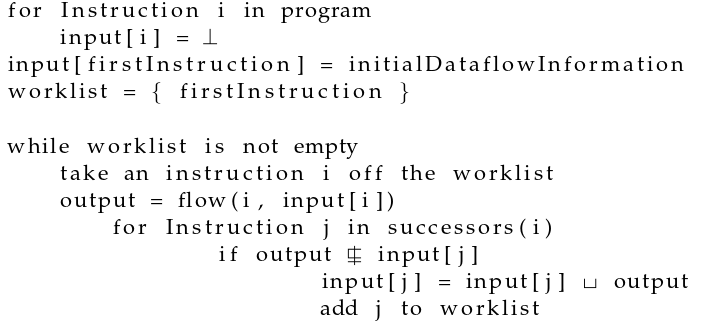
\includegraphics[width=.65\textwidth]{figures/worklist}
  \end{figure}

  \vspace{1em}\pause
  The travelsal order of CFG matters a lot for efficiency!
  The analysis should have processed all predecessors of statement $\mu$
  before processing $\mu$
\end{frame}

%% \section{Termination and Soundness}
%% \frame{\tableofcontents[currentsection]}

%% \begin{frame}

%% \end{frame}

\section{Summary}
\frame{\tableofcontents[currentsection]}

\begin{frame}
  \frametitle{Summary}
  \begin{itemize}
    \item The elements of a Dataflow Analysis\\
      Lattice, Flow Infomation, Flow Function ...
    \item Some applications of Dataflow Analysis
    \item Iterative implementation approach\\
      The Worklist Algorithm
  \end{itemize}
\end{frame}

\begin{frame}
  \frametitle{References}
  \begin{itemize}
    \item Lecture Notes 1--4 of CMU course ``Program Analysis'' (15-819O)\\
      http://www.cs.cmu.edu/~aldrich/courses/15-819O-13sp/
    \item Dataflow Analysis on Wikipedia\\
      http://en.wikipedia.org/wiki/Data-flow\_analysis
  \end{itemize}
\end{frame}

\frame{\centerline{\Huge Q\&A}}

\end{document}
